%% =====================================================================
%%  A_Appendix2.tex --- Appendices for Chapter 4 (Empirical Study)
%% =====================================================================

%% -----------------------------------------------------------------
%%  Appendix B --- AS-IS swimlane with pain points
%% -----------------------------------------------------------------
\chapter{AS-IS process with annotated pain points} \label{app:emp:asis}

This appendix reproduces the AS-IS PO--ASN validation swimlane of Section~\ref{sec:emp:asis}, annotated with the 8 pain point markers from Table~\ref{tab:emp:painpoints}.

\begin{figure}[htbp]
\centering
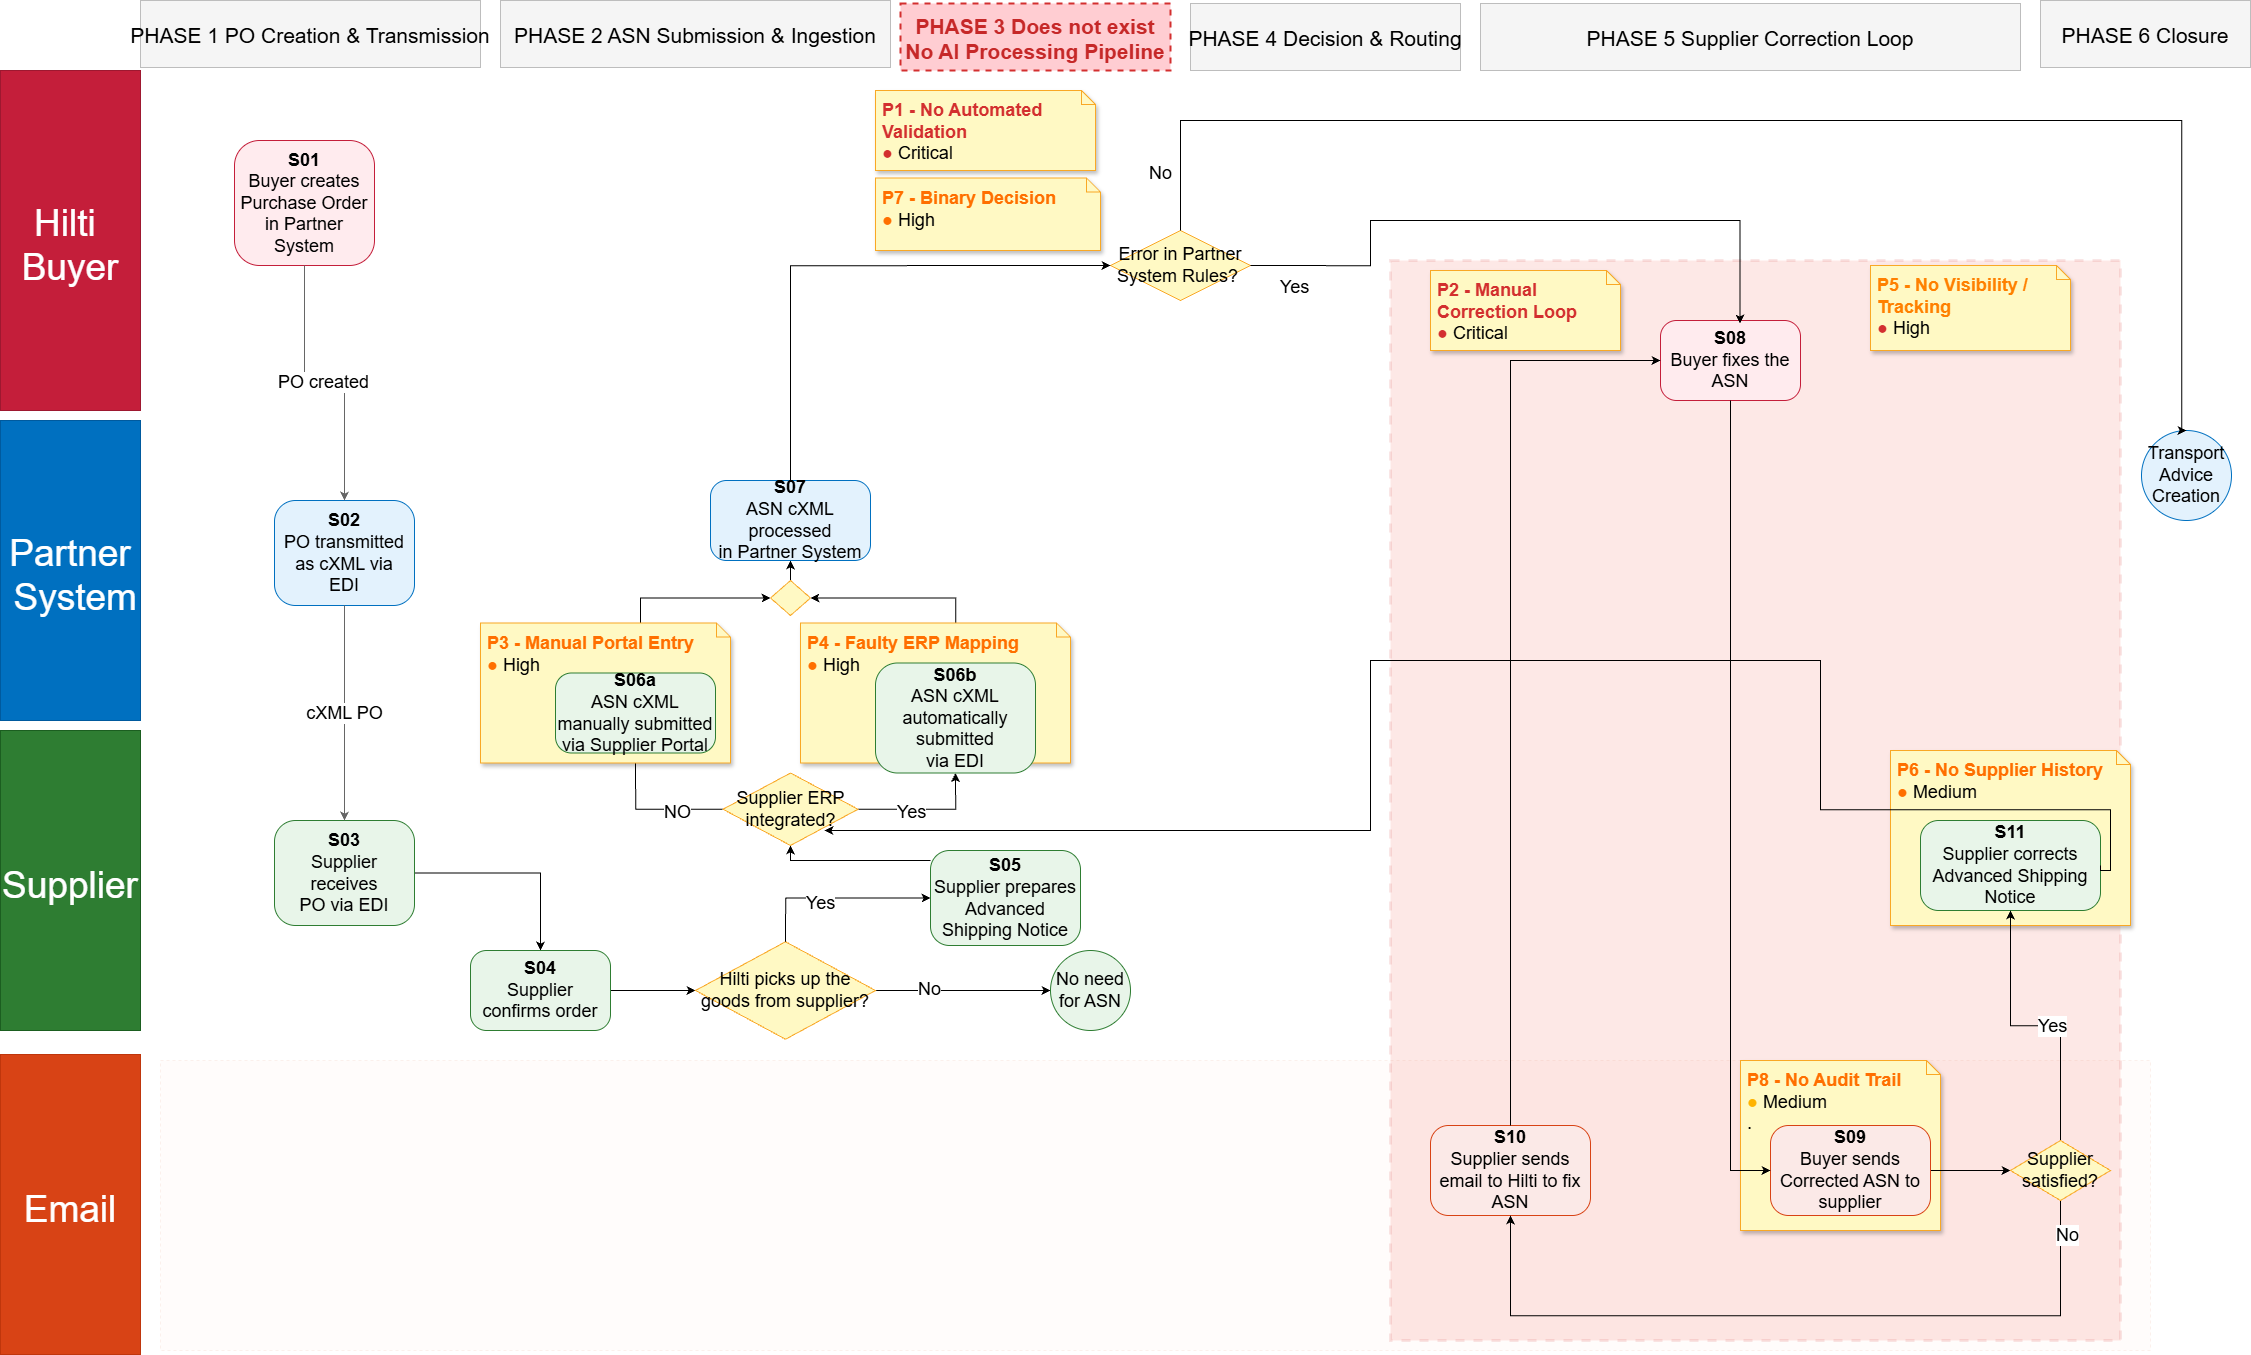
\includegraphics[width=\textwidth]{Figures/fig_4_A_asis_painpoints.png}
\caption{AS-IS process with pain points P1--P8 annotated.}
\label{fig:app:asis}
\end{figure}

The TO-BE process of Section~\ref{sec:emp:tobe} is reproduced below. Phase~3 (AI Processing Pipeline) is inserted between ASN submission and the partner's error check, and an audit log and a key performance indicator dashboard close the learning loop.

\begin{figure}[htbp]
\centering
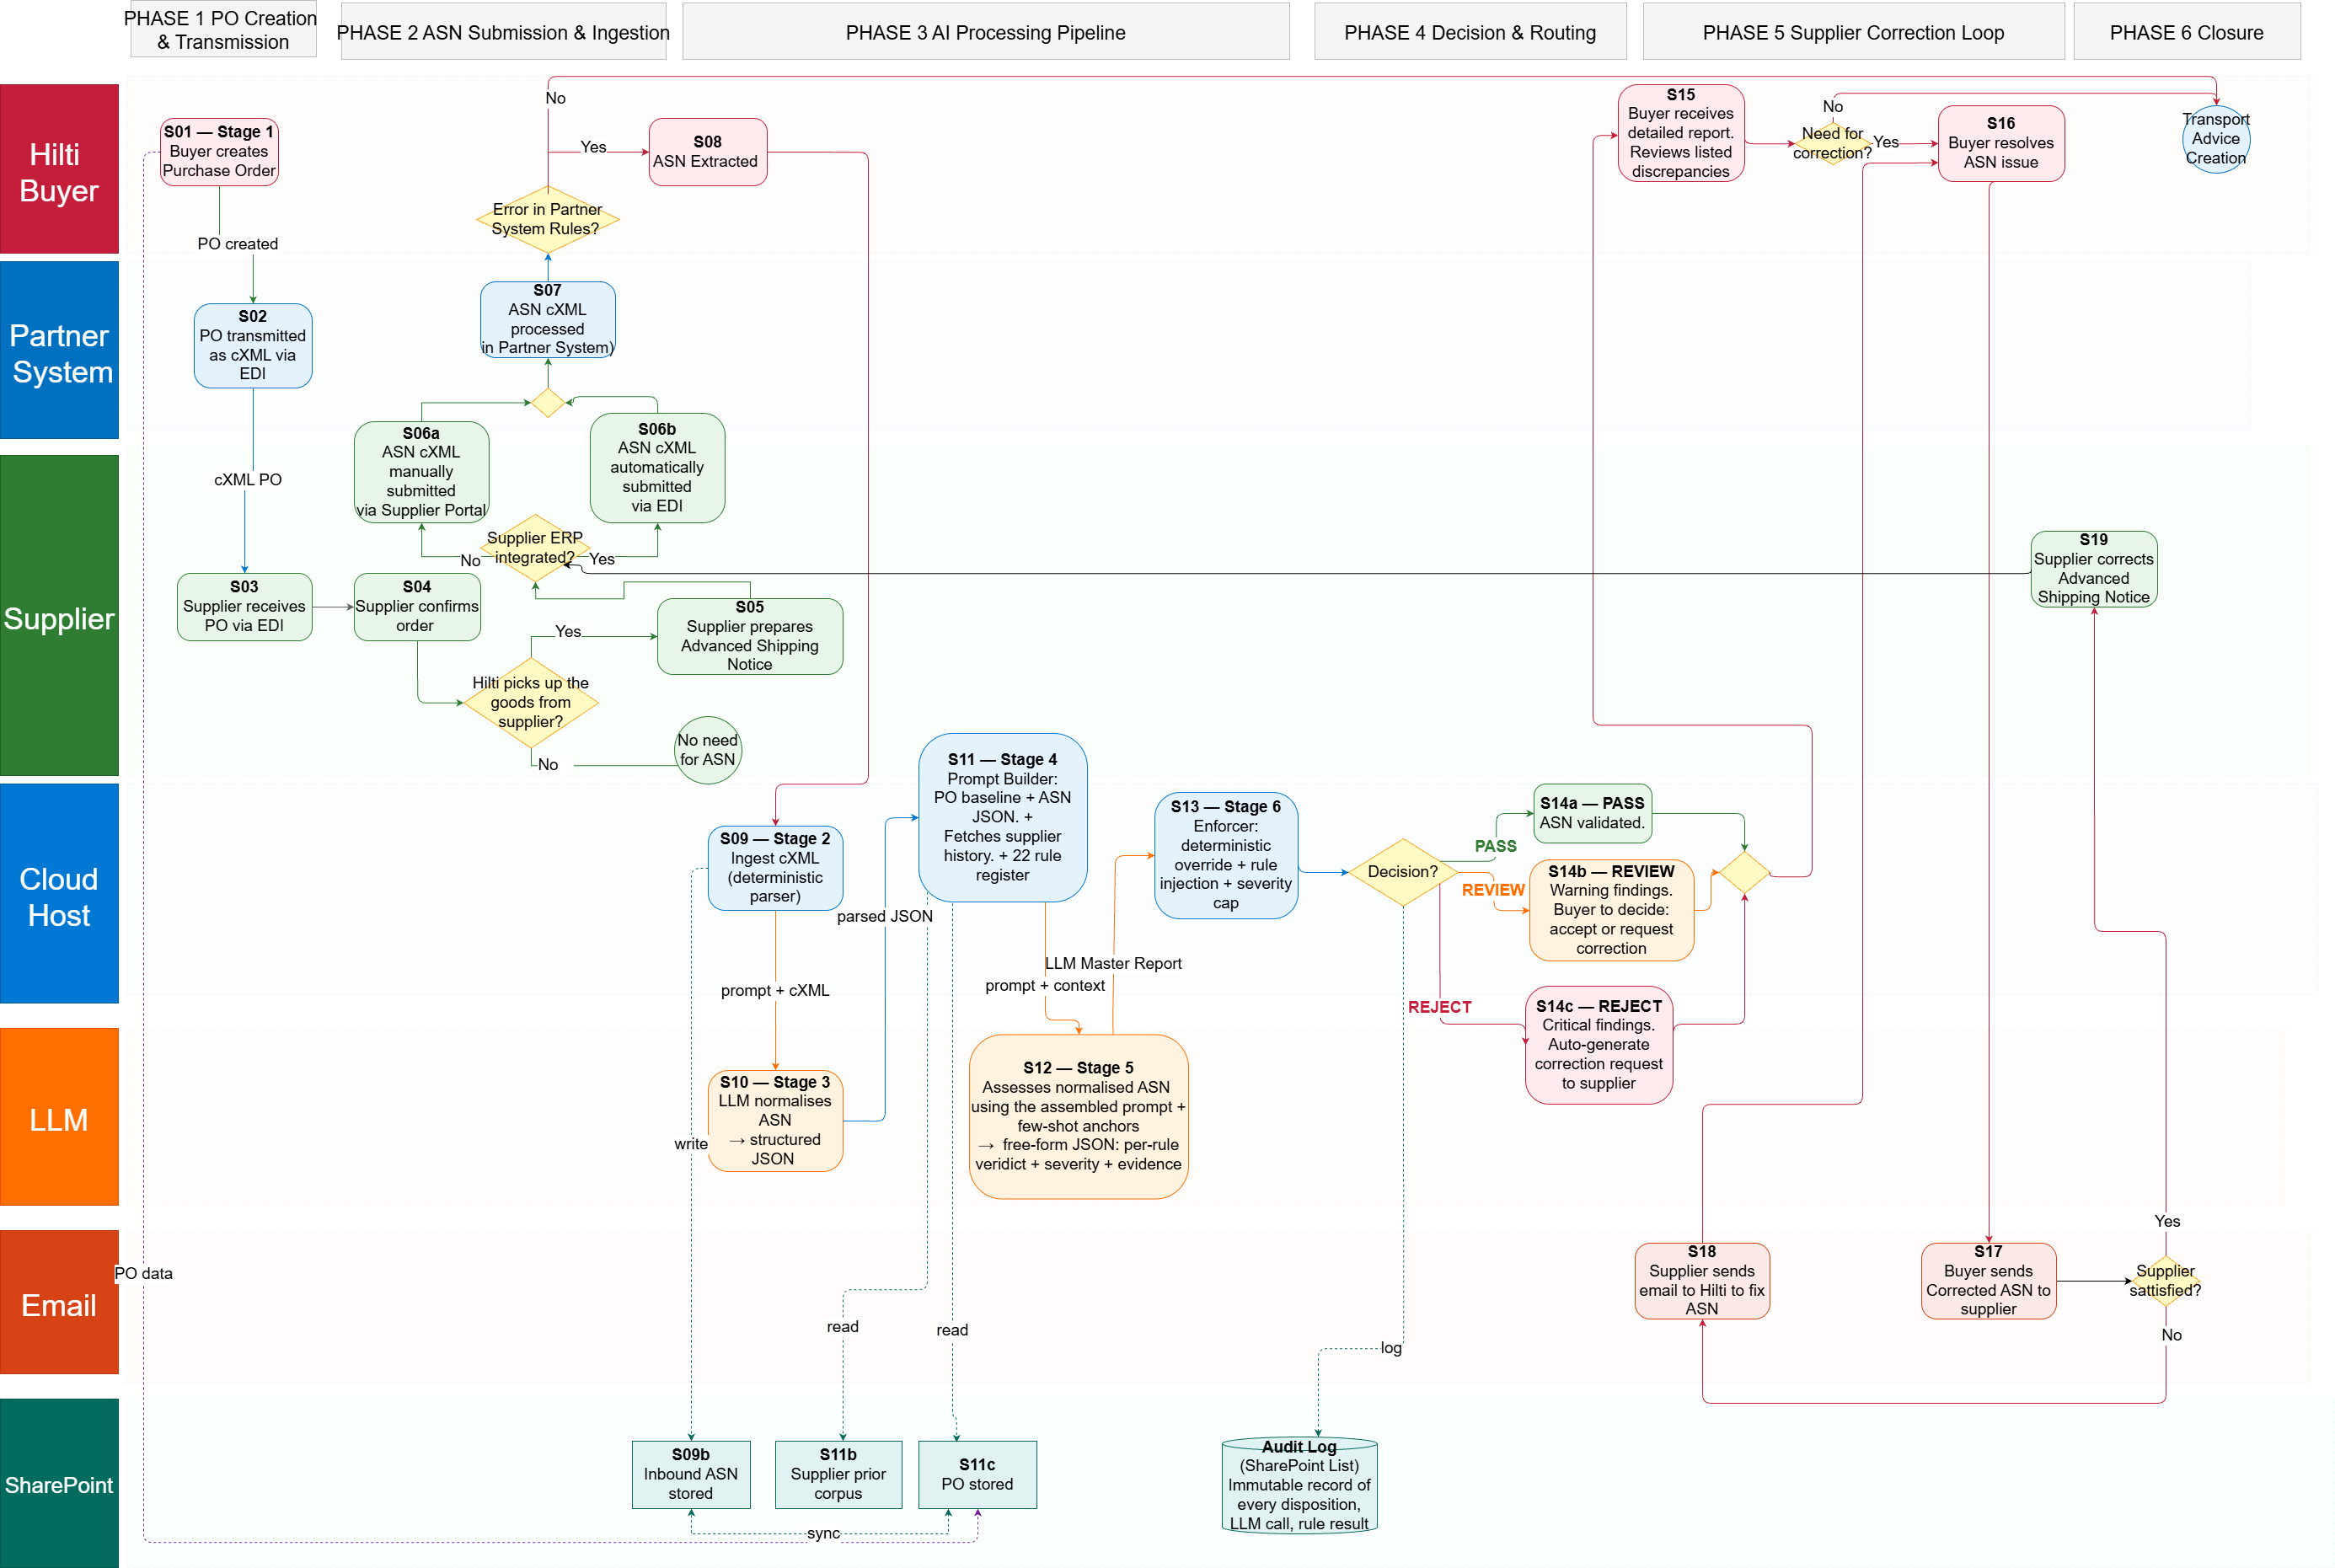
\includegraphics[width=\textwidth]{Figures/fig_4_2_tobe.png}
\caption{TO-BE validation process.}
\label{fig:emp:tobe}
\end{figure}


%% -----------------------------------------------------------------
%%  Appendix C --- Coverage of the rule register by partner static checks
%% -----------------------------------------------------------------
\chapter{Coverage of the rule register by the partner system's static checks} \label{app:emp:coverage}

This appendix maps every rule of the validation register R01--R22 against the static checks the partner system applies at receipt, supporting the claim in Section~\ref{sec:emp:asis} that the partner's coverage of the register is partial and the artefact's contribution is to close the residual gap.

\begin{table}[htbp]
\centering
\caption{Coverage of rules R01--R22 by the partner system's static checks.}
\label{tab:app:coverage}
\scriptsize
\begin{adjustbox}{max width=\textwidth}
\begin{tabular}{@{}lp{5cm}p{5cm}p{4.5cm}@{}}
\toprule
\textbf{Rule} & \textbf{What the rule asks} & \textbf{Covered by static check?} & \textbf{Where the pipeline adds} \\
\midrule
R01 & Quantity not over-shipped vs PO              & Partial --- row~7 catches overflow vs outstanding-to-notify & Severity calibration; REVIEW for partial overflow \\
R02 & Unit price matches PO                        & No                                                          & Pipeline only \\
R03 & Delivery date within tolerance               & Partial --- row~8 catches outside-window                    & REVIEW state for late-but-recoverable \\
R04 & Shipment date not before notice date         & No                                                          & Pipeline only \\
R05 & Unit-of-measure matches PO line              & No --- row~20 only checks dimension consistency             & Pipeline only (PO baseline match) \\
R06 & All PO lines present in ASN                  & No                                                          & Pipeline only \\
R07 & No phantom ASN lines                         & No                                                          & Pipeline only \\
R08 & Currency matches PO                          & No                                                          & Pipeline only \\
R09 & Supplier identity matches PO supplier        & No                                                          & Pipeline only \\
R10 & Each portion references a real PO            & Partial --- row~1 catches line number existence             & Pipeline catches portion-level mismatch \\
R11 & cXML schema compliance                       & Yes --- implicit XML schema validation                      & Recovered for symmetry; redundant on this rule \\
R12 & Mandatory delivery-date attribute present    & No --- row~8 only checks the value if present               & Pipeline catches absence \\
R13 & Transport terms match PO                     & No                                                          & Pipeline only \\
R14 & Ship-To address matches PO                   & No                                                          & Pipeline only \\
R15 & Line total = quantity $\times$ price         & No                                                          & Pipeline only \\
R16 & Partial shipment within tolerance            & Partial --- row~7 catches overflow only                     & Pipeline catches under threshold partials \\
R17 & Line is on the right PO portion              & No                                                          & Pipeline only \\
R18 & No duplicate shipment identifier             & Yes --- row~4                                               & Redundant on this rule \\
R19 & Shipment identifier within 35 characters     & Partial --- row~5, but silently                             & Pipeline catches it loudly, before submission \\
R20 & Gross-to-net weight ratio plausible          & Yes --- rows~11--12                                         & Redundant on this rule, with severity tier \\
R21 & Mandatory packaging block present            & Partial --- rows~16--19                                     & Redundant on this rule, with severity tier \\
R22 & Order not over-fulfilled cumulatively        & Partial --- row~3 catches ``fully shipped'' only            & Pipeline does cumulative shipped quantity tracking \\
\bottomrule
\end{tabular}
\end{adjustbox}
\end{table}

Of the 22 rules in the validation register, 3 (R11, R18 and R20) are fully covered by an existing static check at receipt; 7 (R01, R03, R10, R16, R19, R21 and R22) are partially covered, in the sense that the static check captures one corner of the rule but misses the calibration, the cumulative state, or the loud-versus-silent distinction; and 12 (R02, R04, R05, R06, R07, R08, R09, R12, R13, R14, R15 and R17) are not covered by any static check at all. The 12 uncovered rules are precisely those that compare the ASN against the PO baseline, depend on a supplier's prior history, or require a tiered REVIEW state, 3 classes of validation the partner system does not perform.


%% -----------------------------------------------------------------
%%  Appendix --- Ground truth labelling: checklist and annotation interface
%% -----------------------------------------------------------------
\chapter{Ground truth labelling: checklist and annotation interface} \label{app:emp:annotation}

This appendix details the labelling checklist of Section~\ref{sec:emp:protocol} and the purpose built annotation interface used to apply it, shown in Figure~\ref{fig:emp:annotation}.

\begin{figure}[htbp]
\centering
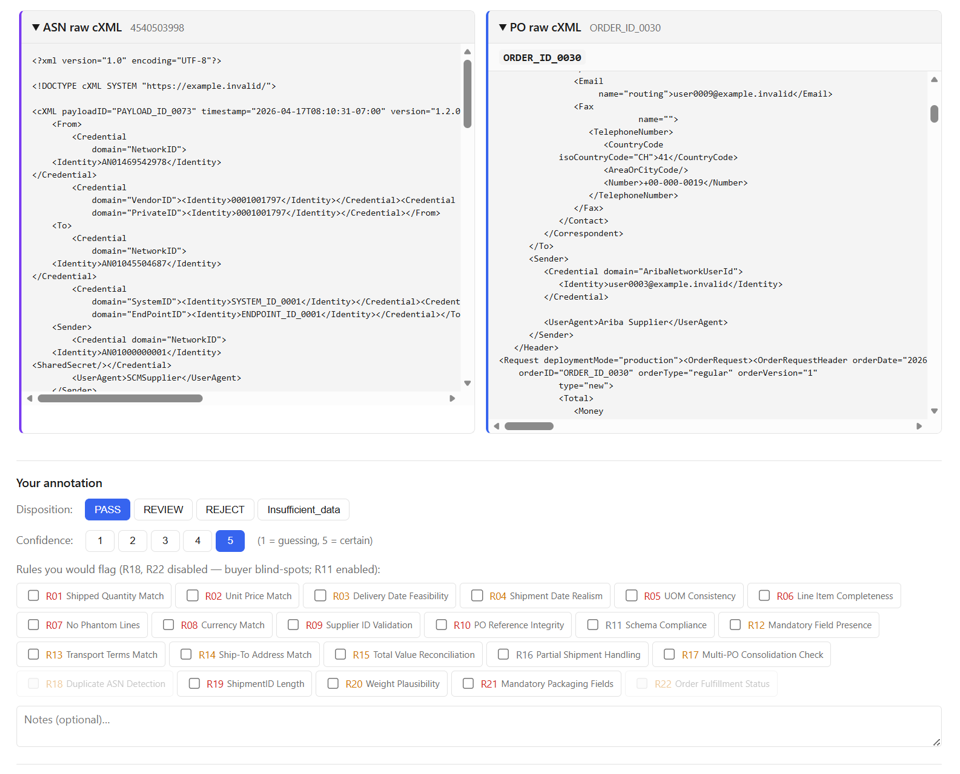
\includegraphics[width=\textwidth]{Figures/fig_D1_annotation.png}

\caption{Annotation interface used during ground truth labelling.}
\label{fig:emp:annotation}
\end{figure}

The interface in Figure~\ref{fig:emp:annotation} removes the per-case overhead the buyer team would otherwise carry: locating the cXML, retrieving the matching PO, opening both in a text editor and transcribing a disposition and a rule list into a spreadsheet. It collapses those steps into a single screen and constrains the analyst to the verdicts the protocol admits. Each case loads with the ASN cXML and the matching PO cXML side by side, both in their raw form, so that the analyst remains close to the document of record and to the evidence the rule register evaluates against.

The annotation panel exposes 4 controls. A disposition selector records the case-level verdict (PASS, REVIEW or REJECT). A 5-point confidence selector records how certain the analyst is of the disposition, on a scale anchored at 1 (guessing) and 5 (certain), and is retained as an audit covariate rather than entering the agreement statistics of Section~\ref{sec:method:eval}. A per rule checklist lets the analyst flag the rules that justify the disposition. A free text notes field captures rationale or edge-case observations that the rule checklist cannot accommodate, and is the source of the failure cluster reasoning in Section~\ref{sec:emp:clustering}.

For every ASN, each analyst labels the rules the checklist exposes as PASS, FAIL or N/A. Two rules are prefilled N/A because neither can be answered from a single ASN card, which leaves 20 rules for the analyst to verdict. R22 (order fulfilment) needs the cumulative shipped quantity across earlier ASNs for the same PO line, and R11 (cXML schema compliance) is an ingestion-time entry check, so a schema-invalid ASN is rejected before it reaches the worksheet and R11 has already passed on every case the analyst sees. R11 and R22 are disabled in the checklist, matching this pre-fill so that the analyst is structurally prevented from labelling cells the protocol cannot answer.

The rules prefilled N/A in labelling are not the same exclusion as the per rule recall denominator of Chapter~\ref{chap:results}. Labelling sets R11 and R22 aside; the recall denominator instead sets R11 and R18 aside, leaving 20 evaluable rules, because R18 (duplicate detection) is exercised by a separate re-submission check rather than by a single ASN verdict. The 2 exclusions are built for different purposes and coincide only on R11.


%% -----------------------------------------------------------------
%%  Appendix E --- Supporting tables for Sections 4.5.4 and 4.5.5
%% -----------------------------------------------------------------
\chapter{Supporting tables for the supplier prior and the real world ground truth} \label{app:emp:supporting}

This appendix gathers the supporting tables for the evaluation set. Table~\ref{tab:emp:blocks} summarises the 3 blocks; Table~\ref{tab:app:percase} lists the buyer ground truth for every real world case in Blocks~A and~B; and Table~\ref{tab:app:perrule} reports the per rule fail rate underlying the prompt sentences of Table~\ref{tab:emp:prompts}.

\begin{table}[htbp]
\centering
\caption{Block summary by source, scope, structural shape and disposition (PASS / REVIEW / REJECT). Referenced from Section~\ref{sec:emp:sources}.}
\label{tab:emp:blocks}
\small
\renewcommand{\arraystretch}{1.3}
\begin{adjustbox}{max width=\textwidth}
\begin{tabular}{@{}llp{3.6cm}rrrc@{}}
\toprule
\textbf{Block} & \textbf{Source} & \textbf{Case range} & \textbf{\# ASNs} & \textbf{\# POs} & \textbf{Multi-PO} & \textbf{Disposition mix} \\
\midrule
A. Production       & Partner platform tracker                  & P-26 to P-61$^{*}$            & 28 & 34  & 3 (11\,\%)  & 4 / 11 / 13 \\
B. Pre-integration  & Same tracker (onboarding flow)            & PI-01 to PI-04                & 4  & 17  & 3 (75\,\%)  & 0 / 4 / 0 \\
C. Synthetic        & Deterministic mutation of clean templates & S-01--S-51, SYN-M01--M17 & 68 & 112 & 11 (16\,\%) & 10 / 23 / 35 \\
\midrule
\textbf{Total} & --- & --- & \textbf{100} & \textbf{163} & \textbf{17 (17\,\%)} & \textbf{14 / 38 / 48} \\
\bottomrule
\end{tabular}
\end{adjustbox}
\par\vspace{0.2em}\footnotesize{$^{*}$ Non-contiguous; gaps are cases removed by the inclusion filter.}
\end{table}

Block~C is summarised here at its full size of 68 cases. One case, S-18 (rule R18, duplicate detection), is tested by a separate re-submission check rather than by a static cXML edit, so it carries no static disposition. The Block~C disposition metrics in Chapter~\ref{chap:results} are therefore reported on the remaining 67 cases.

\begin{table}[htbp]
\centering
\caption{Per-case buyer ground truth on the production and pre-integration sample (32 cases: 4~PASS, 15~REVIEW, 13~REJECT).}
\label{tab:app:percase}
\scriptsize
\begin{adjustbox}{max width=\textwidth}
\begin{tabular}{@{}lllp{2.4cm}p{5.5cm}p{3cm}@{}}
\toprule
\textbf{Case} & \textbf{Block} & \textbf{Supplier} & \textbf{Buyer disposition} & \textbf{Rules flagged} & \textbf{Notes} \\
\midrule
P-26  & A & S2 (CH)  & REJECT  & R02, R08, R13, R14                                  & \\
P-27  & A & S2 (CH)  & REJECT  & R02, R08, R13, R14                                  & \\
P-28  & A & S3 (CH)  & PASS    & ---                                                 & \\
P-29  & A & S3 (CH)  & PASS    & ---                                                 & Timestamp \\
P-30  & A & S3 (CH)  & PASS    & ---                                                 & Timestamp \\
P-31  & A & S5 (US)  & REVIEW  & R03                                                 & Timestamp \\
P-32  & A & S6 (DE)  & PASS    & ---                                                 & Timestamp \\
P-33  & A & S7 (CH)  & REVIEW  & R21 & Timestamp; Multi-PO (3 POs) \\
P-34  & A & S4 (CN)  & REVIEW  & R21                                                 & Timestamp \\
P-35  & A & S4 (CN)  & REVIEW  & R21 & Timestamp; Multi-PO (2 POs) \\
P-36  & A & S1 (AT)  & REJECT  & R02, R05, R08, R13, R14                             & \\
P-37  & A & S1 (AT)  & REJECT  & R13, R14                                            & \\
P-38  & A & S1 (AT)  & REJECT  & R02, R06, R12, R14, R21                             & \\
P-39  & A & S1 (AT)  & REJECT  & R02, R06, R12, R13, R14                             & \\
P-40  & A & S1 (AT)  & REJECT  & R02, R06, R12, R13, R14                             & \\
P-41  & A & S1 (AT)  & REJECT  & R06, R12, R13, R14                                  & \\
P-42  & A & S1 (AT)  & REJECT  & R02, R05, R06, R08, R12, R13, R14                   & \\
P-43  & A & S1 (AT)  & REJECT  & R02, R05, R06, R08, R12, R13, R14                   & \\
P-44  & A & S1 (AT)  & REJECT  & R08, R14, R21                                       & \\
P-45  & A & S12 (CZ) & REVIEW  & R03, R06, R13, R14, R21 & \\
P-48  & A & S12 (CZ) & REVIEW  & R03, R06, R13, R14, R21 & Multi-PO (4 POs) \\
P-51  & A & S13 (CH) & REJECT  & R03, R08, R13, R14, R21                             & \\
P-54  & A & S17 (CH) & REVIEW  & R03, R13, R14, R21                                  & \\
P-55  & A & S18 (HU) & REVIEW  & R13, R14, R21                                       & \\
P-57  & A & S19 (CH) & REVIEW  & R03, R06, R13, R14, R21                             & \\
P-58  & A & S20 (IT) & REVIEW  & R03, R13, R14, R21                                  & \\
P-59  & A & S20 (IT) & REJECT  & R08, R13, R14, R21                                  & \\
P-61  & A & S21 (DE) & REVIEW  & R13, R14, R21                                       & \\
PI-01 & B & S8 (GB)  & REVIEW  & R03, R13, R14, R21                                  & Multi-PO (8 POs) \\
PI-02 & B & S9 (AT)  & REVIEW  & R13, R14, R21                                       & Multi-PO (3 POs) \\
PI-03 & B & S10 (BE) & REVIEW  & R13, R14, R21                                       & Single-PO \\
PI-04 & B & S11 (DE) & REVIEW  & R03, R06, R13, R14, R21                             & Multi-PO (5 POs) \\
\bottomrule
\end{tabular}
\end{adjustbox}
\end{table}

\begin{table}[htbp]
\centering
\caption{Per rule fail rate by supplier on the prior corpus. Cells are blank where no firing was recorded; only the 8 rules active in the corpus are shown.}
\label{tab:app:perrule}
\footnotesize
\begin{adjustbox}{max width=\textwidth}
\begin{tabular}{@{}lcccccccc@{}}
\toprule
\textbf{Supplier} & \textbf{R02} & \textbf{R03} & \textbf{R06} & \textbf{R08} & \textbf{R12} & \textbf{R13} & \textbf{R14} & \textbf{R21} \\
\midrule
S1 (AT)  & 0.67 & ---  & 0.67 & 0.44 & 0.67 & 0.78 & 1.00 & 0.22 \\
S2 (CH)  & 1.00 & ---  & ---  & 1.00 & ---  & 1.00 & 1.00 & ---  \\
S3 (CH)  & ---  & ---  & ---  & ---  & ---  & ---  & ---  & ---  \\
S4 (CN)  & ---  & ---  & ---  & ---  & ---  & ---  & ---  & ---  \\
S12 (CZ) & ---  & 1.00 & 1.00 & ---  & ---  & 1.00 & 1.00 & 1.00 \\
\bottomrule
\end{tabular}
\end{adjustbox}
\end{table}

\begin{table}[htbp]
\centering
\caption{The 5 supplier prompt lines. Sentences are shown for the full corpus, after the pipeline's evaluation sweep.}
\label{tab:emp:prompts}
\scriptsize
\begin{adjustbox}{max width=\textwidth}
\begin{tabular}{@{}llp{8.2cm}p{4.2cm}@{}}
\toprule
\textbf{Supplier} & \textbf{Prior} & \textbf{Prompt sentence} & \textbf{Intent} \\
\midrule
S1 (AT) & REJECT &
``Historical note: this supplier has failed R14 in 9/9, R13 in 7/9, R02 in 6/9 prior ASN(s). Pay extra attention to those checks.'' &
Lean toward REJECT on address, transport and price. \\
\addlinespace
S2 (CH) & REJECT &
``Historical note: this supplier has failed R02 in 2/2, R08 in 2/2, R13 in 2/2 prior ASN(s). Pay extra attention to those checks.'' &
Lean toward REJECT on price, currency and transport. \\
\addlinespace
S3 (CH) & PASS &
``Historical note: the buyer has validated all 3 prior ASN(s) from this supplier as PASS (zero rule failures recorded). Note: 2/3 prior ASN(s) failed upstream in SAP due to a known order confirmation timestamp bug, and those should pass under current rules; do not let the historical failure count inflate REVIEW/REJECT signals for this supplier on similar cases.'' &
Ignore the visible failure history; it is a platform artefact. \\
\addlinespace
S4 (CN) & REVIEW &
``Historical note: this supplier has 2 prior ASN(s) on file, both REVIEW (R21 missing packaging). The prior failures coincide with a known order-confirmation timestamp bug in SAP; weigh content-level evidence above the timestamp signal.'' &
Read R21 as the genuine signal; do not over-attribute to the platform artefact. \\
\addlinespace
S12 (CZ) & REVIEW &
``Historical note: this supplier has failed R03 in 2/2, R06 in 2/2, R13 in 2/2 prior ASN(s). Pay extra attention to those checks.'' &
Watch delivery date, partial delivery and transport. \\
\bottomrule
\end{tabular}
\end{adjustbox}
\end{table}


\clearpage
\section*{Full synthetic perturbation inventory (S-01 to S-51)}

Table~\ref{tab:app:mutants_full} enumerates the 51 single rule synthetic mutants of Block~C, reported per case with target rule, design group, expected disposition, collateral rules and the cXML edit applied. Mutants S-01 to S-22 each target a single rule across the register R01 to R22; mutants S-23 to S-51 extend the block along the three design groups introduced in Section~\ref{sec:emp:synthetic}: boundary, magnitude and mechanism, and supplier diversity.

\footnotesize
\begin{longtable}{@{}llllp{6.5cm}@{}}
\caption{Full synthetic perturbation inventory: S-01 to S-51 single rule mutants.}\label{tab:app:mutants_full}\\
\toprule
\textbf{Case} & \textbf{Target} & \textbf{Group} & \textbf{Expected} & \textbf{cXML edit applied} \\
\midrule
\endfirsthead
\toprule
\textbf{Case} & \textbf{Target} & \textbf{Group} & \textbf{Expected} & \textbf{cXML edit applied} \\
\midrule
\endhead
\midrule
\multicolumn{5}{r}{\emph{Continued on next page}} \\
\endfoot
\bottomrule
\endlastfoot
S-01 & R01 & Base & REJECT & Quantity 2016 $\to$ 3000 (49\,\% over-fulfilment, 0\,\% tolerance) \\
S-02 & R02 & Base & REJECT & Unit price 2.26 $\to$ 5.00 \\
S-03 & R03 & Base & REVIEW & Delivery date 49 days late \\
S-04 & R04 & Base & REVIEW & Shipment date set before notice date \\
S-05 & R05 & Base & REJECT & UOM H87 $\to$ KGM (PO expects H87) \\
S-06 & R06 & Base & REVIEW & Removed ShipNoticeItem line=10 \\
S-07 & R07 & Base & REJECT & Phantom ShipNoticeItem line=99 \\
S-08 & R08 & Base & REJECT & Currency EUR $\to$ USD \\
S-09 & R09 & Base & REJECT & Supplier NetworkID 0014 $\to$ 0015 \\
S-10 & R10 & Base & REJECT & Added second portion against non-existent PO \\
S-11 & ---  & Base (PASS) & PASS & Clean ASN, schema valid (R11 PASS control) \\
S-12 & R12 & Base & REVIEW & Removed deliveryDate attribute \\
S-13 & R13 & Base & REVIEW & Transport terms FCA $\to$ DDP \\
S-14 & R14 & Base & REVIEW & Ship-To addressID 0524 $\to$ 9999 \\
S-15 & R15 & Base & REJECT & Line total inconsistent with quantity $\times$ price \\
S-16 & R16 & Base & REVIEW & Quantity 2016 $\to$ 1000 (50\,\% partial shipment) \\
S-17 & R17 & Base & REVIEW & Line moved to wrong PO portion \\
S-18$^{\dagger}$ & R18 & Base (nominal) & REVIEW & Duplicate shipment identifier check (sequential re-submission, not a static edit) \\
S-19 & R19 & Base & REJECT & Shipment identifier 42 characters (limit 35) \\
S-20 & R20 & Base & REVIEW & Gross / net weight ratio above $100\times$ \\
S-21 & R21 & Base & REJECT & Removed all packaging dimensions \\
S-22 & R22 & Base & REJECT & Quantity 2016 $\to$ 4032 (2$\times$ PO quantity) \\
\midrule
S-23 & --- & Boundary (PASS) & PASS  & Just inside PASS control \\
S-24 & --- & Boundary (PASS) & PASS  & Just inside PASS control \\
S-25 & --- & Boundary (PASS) & PASS  & Just inside PASS control (R20 ratio exactly at 10.0) \\
S-26 & --- & Boundary (PASS) & PASS  & Just inside PASS control \\
S-27 & --- & Boundary (PASS) & PASS  & Just inside PASS control \\
S-28 & --- & Boundary (PASS) & PASS  & Just inside PASS control \\
S-29 & R03 & Boundary        & REVIEW & R03 delivery window edge case \\
S-30 & R03 & Boundary        & REVIEW & R03 delivery window edge case \\
S-31 & R19 & Boundary        & REJECT & R19 35 character limit edge case \\
S-32 & R20 & Boundary        & REVIEW & R20 weight ratio edge case \\
S-33 & R01 & Boundary        & REJECT & R01 zero tolerance tightest margin \\
S-34 & R02 & Boundary        & REJECT & R02 zero tolerance tightest margin \\
\midrule
S-35 & R16 & Magnitude/mechanism        & REVIEW & R16 partial shipment, alternative magnitude \\
S-36 & R02 & Magnitude/mechanism        & REJECT & R02 under pricing variant \\
S-37 & R05 & Magnitude/mechanism (PASS) & PASS   & R05 canonical equivalent UOM (PASS control) \\
S-38 & R06 & Magnitude/mechanism        & REJECT & R06 full-miss critical variant \\
S-39 & R08 & Magnitude/mechanism        & REJECT & R08 line-level currency mismatch \\
S-40 & R09 & Magnitude/mechanism (PASS) & PASS   & R09 VendorID only (PASS control) \\
S-41 & R13 & Magnitude/mechanism        & REVIEW & R13 \texttt{value="Other"} text path \\
S-42 & R21 & Magnitude/mechanism        & REVIEW & R21 net-only missing dimension variant \\
S-43 & R21 & Magnitude/mechanism        & REVIEW & R21 type only missing dimension variant \\
S-44 & R12 & Magnitude/mechanism        & REVIEW & R12 missing line number variant \\
\midrule
S-45 & R08 & Supplier diversity (template C)   & REJECT & R08 currency mismatch on template C \\
S-46 & R02 & Supplier diversity (template C)   & REJECT & R02 unit price mismatch on template C \\
S-47 & R03 & Supplier diversity (template C)   & REVIEW & R03 late delivery on template C \\
S-48 & R21 & Supplier diversity (template C)   & REVIEW & R21 missing packaging on template C \\
S-49 & R02 & Supplier diversity (template D) & REJECT & R02 unit price mismatch on template D \\
S-50 & R08 & Supplier diversity (template D) & REJECT & R08 currency mismatch on template D \\
S-51 & R03 & Supplier diversity (template D) & REVIEW & R03 late delivery on template D \\
\end{longtable}
\par\vspace{0.2em}\footnotesize{$^{\dagger}$ Tested by a separate re-submission check, not a static cXML edit; excluded from the Chapter~\ref{chap:results} disposition cohort.}
\normalsize

\begin{table}[htbp]
\centering
\caption{Multi-rule synthetic scenarios (Block~C, multi-rule subset, SYN-M01 to SYN-M17).}
\label{tab:app:multirule}
\footnotesize
\begin{adjustbox}{max width=\textwidth}
\begin{tabular}{@{}lp{6.5cm}ll@{}}
\toprule
\textbf{Case} & \textbf{Combined defects} & \textbf{Target rules} & \textbf{Expected} \\
\midrule
SYN-M01 & Over-shipment + currency mismatch + missing packaging                & R01, R08, R21   & REJECT \\
SYN-M02 & Late delivery + UOM mismatch + wrong supplier identifier             & R03, R05, R09   & REJECT \\
SYN-M03 & Unit price mismatch + phantom ASN line                               & R02, R07        & REJECT \\
SYN-M04 & Partial shipment + wrong transport terms                             & R13, R16        & REVIEW \\
SYN-M05 & Line total inconsistency + over length shipment ID + missing packaging & R15, R19, R21 & REJECT \\
SYN-M06 & Quantity over shipment + line total inconsistency                    & R01, R15        & REJECT \\
SYN-M07 & Quantity over shipment + currency mismatch                           & R01, R08        & REJECT \\
SYN-M08 & Phantom ASN line + wrong transport terms                             & R07, R13        & REJECT \\
SYN-M09 & Quantity + unit price + line total errors compounded                 & R01, R02, R15   & REJECT \\
SYN-M10 & Partial shipment + missing packaging                                 & R16, R21        & REJECT \\
SYN-M11 & Currency mismatch + wrong transport terms                            & R08, R13        & REJECT \\
SYN-M12 & Late delivery + wrong transport terms                                & R03, R13        & REVIEW \\
SYN-M13 & Multi-rule PASS control (no defects)                                 & ---             & PASS   \\
SYN-M14 & UOM mismatch + partial shipment                                      & R05, R16        & REJECT \\
SYN-M15 & Currency mismatch + over length shipment ID + missing packaging      & R08, R19, R21   & REJECT \\
SYN-M16 & Unit price mismatch + wrong supplier identifier                      & R02, R09        & REJECT \\
SYN-M17 & Quantity over shipment + late delivery + wrong transport terms       & R01, R03, R13   & REJECT \\
\bottomrule
\end{tabular}
\end{adjustbox}
\end{table}


\chapter{Operational measurements}
\label{app:operational}

This appendix reports the full operational spread per pipeline design on the 28 production evaluation cases per design. The headline figures, median latency and mean cost per ASN, are cited in Chapter~\ref{chap:results}, Section~\ref{sec:results:cost}; the full descriptive spread is reported here.

\begin{table}[htbp]
\centering
\caption{Operational spread per design on the 28 production evaluation cases per design. Costs are in euros. Q1 and Q3 are the lower and upper quartiles; p90 and p95 are the values below which 90\% and 95\% of cases fall. The 99th percentile is omitted because with 28 cases it collapses onto the maximum.}
\label{tab:app:operational}
\footnotesize
\setlength{\tabcolsep}{4pt}

\begin{adjustbox}{max width=\textwidth}
\begin{tabular}{@{}lrrrrrrrr@{}}
\multicolumn{9}{l}{\textbf{Latency per ASN (seconds)}} \\
\toprule
\textbf{Design} & \textbf{Min} & \textbf{Q1} & \textbf{Median} & \textbf{Q3} & \textbf{p90} & \textbf{p95} & \textbf{Max} & \textbf{StdDev} \\
\midrule
pure LLM      & 10.65 & 11.88 & 13.14 & 15.74 & 20.00 & 32.30 & 34.98 & 5.70 \\
post hoc      & 10.58 & 12.13 & 13.94 & 16.19 & 21.77 & 30.09 & 36.22 & 5.81 \\
LLM-as-judge  & 12.04 & 12.85 & 13.67 & 16.72 & 23.24 & 35.19 & 38.33 & 7.04 \\
in generation & 9.10  & 11.37 & 13.22 & 16.94 & 23.22 & 33.81 & 48.47 & 7.93 \\
pre hoc       & 7.05  & 7.48  & 7.89  & 9.45  & 10.11 & 12.27 & 15.38 & 1.73 \\
\bottomrule
\end{tabular}
\end{adjustbox}

\medskip

\begin{adjustbox}{max width=\textwidth}
\begin{tabular}{@{}lrrrrrr@{}}
\multicolumn{7}{l}{\textbf{Tokens and cost per ASN}} \\
\toprule
\textbf{Design} & \textbf{Prompt mean} & \textbf{Completion mean} & \textbf{Cost mean (EUR)} & \textbf{Cost p95} & \textbf{Cost max} & \textbf{Cost StdDev} \\
\midrule
pure LLM      & 12{,}615 & 3{,}723 & 0.109 & 0.201 & 0.500 & 0.080 \\
post hoc      & 12{,}614 & 3{,}838 & 0.111 & 0.203 & 0.502 & 0.081 \\
LLM-as-judge  & 15{,}859 & 3{,}931 & 0.127 & 0.247 & 0.518 & 0.086 \\
in generation & 26{,}244 & 3{,}662 & 0.171 & 0.351 & 0.563 & 0.100 \\
pre hoc       & 9{,}870  & 1{,}970 & 0.073 & 0.111 & 0.463 & 0.075 \\
\bottomrule
\end{tabular}
\end{adjustbox}
\end{table}

\paragraph{Annual volume basis for the cost projection.} The cost projection in Section~\ref{sec:results:cost} scales the per-case handling time by the live ASN volume. In a representative month of live production the function processed 2,331 unique ASNs, of which 51 failed validation, a fail rate of about 2 per cent; this is of the order of 28,000 ASNs and 610 failed ASNs per year. Each failed ASN triggers the 30 to 90 minute correction loop, and 2 factors raise the per-case time above a single document handled by one buyer. First, the buyer opens and compares the ASN against each PO it references, so the time scales with the number of documents handled; the production sample averages 1.48 referenced POs per ASN, with 21 per cent referencing more than one, so an average case handles about 2.48 documents against 2 for a single-PO case, a measured uplift of about a quarter (a factor of 1.24). Second, a buyer without spare capacity escalates a case to colleagues, so a case is sometimes worked by more than one buyer; no escalation rate is recorded, so a conservative factor of 1.5 is assumed and is flagged as an assumption rather than a measurement. Applying both factors to the 610 failed ASNs per year at 30 to 90 minutes each gives of the order of 570 to 1,700 analyst hours per year.

\paragraph{Hourly cost basis for the labour saving estimate.} The labour saving in Section~\ref{sec:concl:practice} values the analyst hours removed at the loaded hourly cost of a materials manager at the partner organisation, about EUR 38 per hour. This is derived from an annual salary of roughly EUR 82,000, spread over 13 payments, 4 working weeks per month and 41.75 working hours per week. Multiplying the estimated 570 to 1,700 analyst hours per year by this rate gives the order of EUR 22,000 to 65,000 per year.

\begin{figure}[htb]
\centering
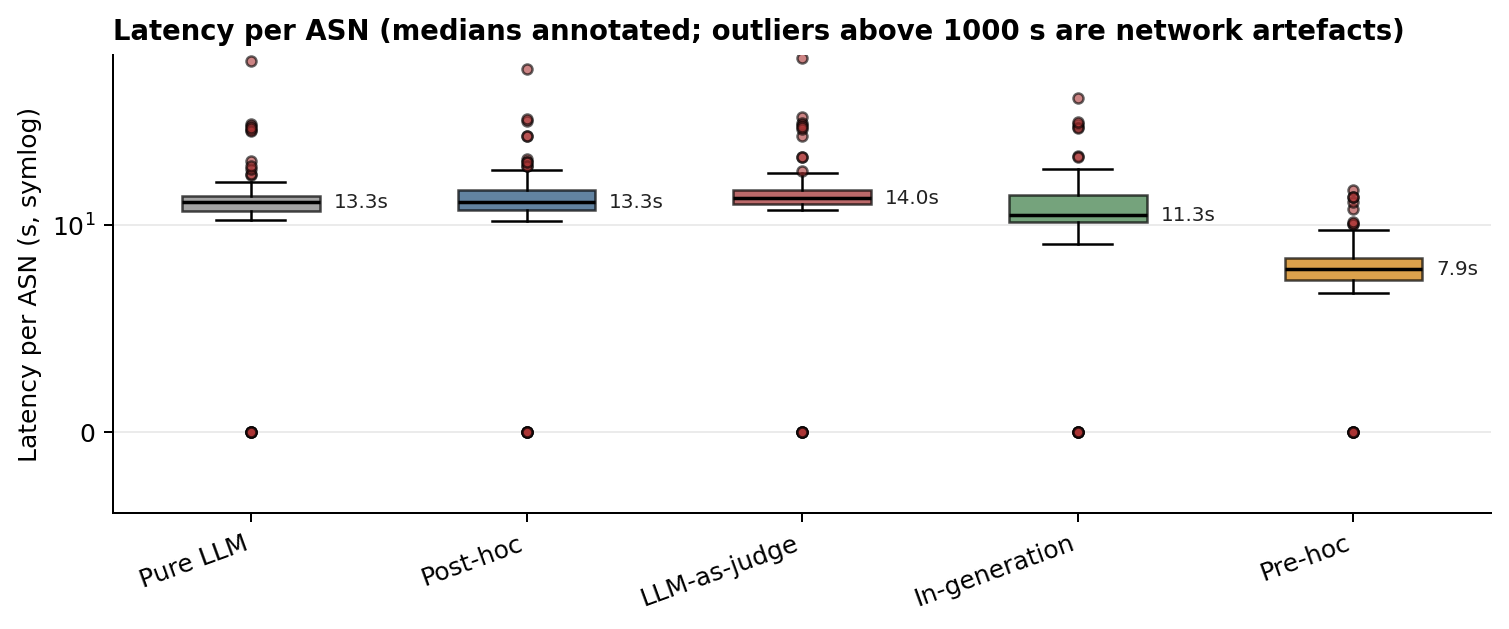
\includegraphics[width=0.82\textwidth]{Figures/fig_5_5_latency_box.png}
\caption{Latency per ASN by design (box = interquartile range, line = median, points = provider-delay outliers). Referenced from Section~\ref{sec:results:cost}.}
\label{fig:results:latency}
\end{figure}

\begin{figure}[htb]
\centering
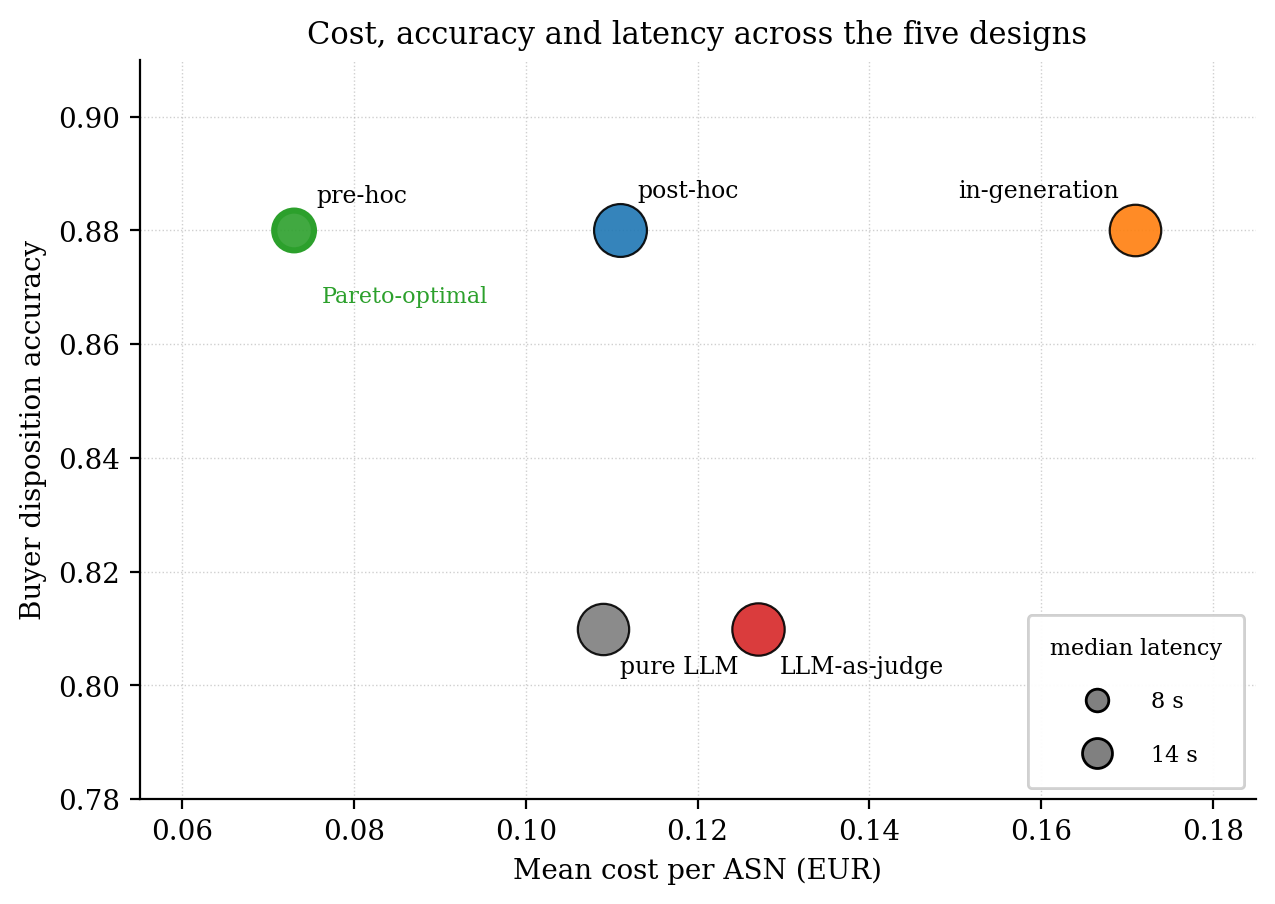
\includegraphics[width=0.78\textwidth]{Figures/fig_5_pareto.png}
\caption{Cost and latency on the 28 production cases and accuracy on the 32 buyer cases; marker area is median latency. Referenced from Section~\ref{sec:results:cost}.}
\label{fig:results:pareto}
\end{figure}


%% -----------------------------------------------------------------
%%  Appendix: Full disposition metrics (Chapter 5)
%% -----------------------------------------------------------------
\chapter{Full disposition metrics}
\label{app:dispmetrics}

This appendix reports the point estimates and 95 per cent bootstrap confidence intervals for all 4 disposition metrics, on both samples. The bar chart of Figure~\ref{fig:results:metrics} in Chapter~\ref{chap:results} summarises these values; the full table is given here.

\begin{table}[htbp]
\centering
\caption{Disposition agreement and per rule recall on the synthetic cohort (67 cases). 95 per cent bootstrap intervals in brackets; recall is over the 41 evaluable single rule mutant targets.}
\label{tab:app:dispsynth}
\footnotesize
\begin{adjustbox}{max width=\textwidth}
\begin{tabular}{@{}lccccc@{}}
\toprule
\textbf{Design} & \textbf{Accuracy} & \textbf{Weighted F1} & \textbf{Weighted kappa} & \textbf{Gwet AC2} & \textbf{Rule recall} \\
\midrule
pure LLM      & 0.81 [0.70, 0.90] & 0.80 [0.70, 0.89] & 0.78 [0.63, 0.90]        & 0.79 [0.68, 0.90] & 29/41 = 0.71 \\
post hoc      & 0.87 [0.78, 0.94] & 0.87 [0.78, 0.94] & 0.86 [0.77, 0.94]        & 0.87 [0.78, 0.94] & 37/41 = 0.90 \\
LLM-as-judge  & 0.51 [0.37, 0.64] & 0.42 [0.28, 0.57] & $-$0.01 [$-$0.12, 0.13]  & 0.49 [0.30, 0.65] & 26/41 = 0.63 \\
in generation & 0.84 [0.75, 0.91] & 0.84 [0.75, 0.91] & 0.80 [0.65, 0.91]        & 0.82 [0.71, 0.92] & 28/41 = 0.68 \\
pre hoc       & 0.88 [0.79, 0.96] & 0.88 [0.79, 0.95] & 0.88 [0.79, 0.95]        & 0.88 [0.80, 0.95] & 40/41 = 0.98 \\
\bottomrule
\end{tabular}
\end{adjustbox}
\end{table}

\begin{table}[htbp]
\centering
\caption{Disposition agreement and per rule recall on the buyer sample (32 cases, 28 production and 4 pre-integration). 95 per cent bootstrap intervals in brackets.}
\label{tab:app:dispbuyer}
\footnotesize
\begin{adjustbox}{max width=\textwidth}
\begin{tabular}{@{}lccccc@{}}
\toprule
\textbf{Design} & \textbf{Accuracy} & \textbf{Weighted F1} & \textbf{Weighted kappa} & \textbf{Gwet AC2} & \textbf{Rule recall} \\
\midrule
pure LLM      & 0.81 [0.66, 0.94] & 0.80 [0.64, 0.94] & 0.78 [0.58, 0.93] & 0.82 [0.68, 0.94] & 40/106 = 0.38 \\
post hoc      & 0.88 [0.75, 0.97] & 0.82 [0.65, 0.95] & 0.82 [0.69, 0.94] & 0.88 [0.75, 0.97] & 55/106 = 0.52 \\
LLM-as-judge  & 0.81 [0.66, 0.94] & 0.76 [0.58, 0.92] & 0.75 [0.60, 0.89] & 0.83 [0.68, 0.95] & 43/106 = 0.41 \\
in generation & 0.88 [0.75, 0.97] & 0.82 [0.65, 0.95] & 0.82 [0.69, 0.94] & 0.88 [0.75, 0.97] & 43/106 = 0.41 \\
pre hoc       & 0.88 [0.75, 0.97] & 0.82 [0.65, 0.95] & 0.82 [0.69, 0.94] & 0.88 [0.75, 0.97] & 51/106 = 0.48 \\
\bottomrule
\end{tabular}
\end{adjustbox}
\end{table}

\begin{table}[htbp]
\centering
\caption{Severity-weighted macro F1 by rule regime (fail = positive class; severity weights 1/2/3). Parentheses give the contributing rules. Referenced from Section~\ref{sec:results:regimes}.}
\label{tab:results:fwslices}
\footnotesize
\begin{adjustbox}{max width=\textwidth}
\begin{tabular}{@{}lcccccc@{}}
\toprule
& \multicolumn{3}{c}{\textbf{Synthetic}} & \multicolumn{3}{c}{\textbf{Buyer}} \\
\cmidrule(lr){2-4} \cmidrule(lr){5-7}
\textbf{Design} & \textbf{Det.\ (8)} & \textbf{LM (14)} & \textbf{All (22)} & \textbf{Det.\ (8)} & \textbf{LM (14)} & \textbf{All (22)} \\
\midrule
pure LLM      & 0.598 (7) & 0.620 (13) & 0.613 (20) & 0.386 (5) & 0.272 (8)  & 0.318 (13) \\
post hoc      & 0.701 (7) & 0.593 (13) & 0.631 (20) & 0.442 (6) & 0.340 (8)  & 0.384 (14) \\
LLM-as-judge  & 0.486 (8) & 0.332 (13) & 0.390 (21) & 0.351 (7) & 0.172 (11) & 0.244 (18) \\
in generation & 0.715 (7) & 0.572 (13) & 0.622 (20) & 0.410 (6) & 0.346 (8)  & 0.374 (14) \\
pre hoc       & 0.702 (7) & 0.694 (13) & 0.697 (20) & 0.437 (6) & 0.189 (8)  & 0.293 (14) \\
\bottomrule
\end{tabular}
\end{adjustbox}
\end{table}

\begin{table}[htbp]
\centering
\caption{Enforcer actions per design. The severity-cap column counts markers; distinct cases are 4 (LLM-as-judge) and 6 (in generation), used in Table~\ref{tab:results:capping}. R16 escalations and downgrades were 0 throughout. Referenced from Section~\ref{sec:results:actions}.}
\label{tab:results:actions}
\footnotesize
\begin{tabular}{@{}lccc@{}}
\toprule
\textbf{Design} & \textbf{Override} & \textbf{Injection} & \textbf{Severity cap (markers)} \\
\midrule
pure LLM      & 0  & 0  & 0  \\
post hoc      & 32 & 43 & 0  \\
LLM-as-judge  & 0  & 0  & 4  \\
in generation & 0  & 0  & 10 \\
pre hoc       & 0  & 0  & 0  \\
\bottomrule
\end{tabular}
\end{table}

\begin{table}[htbp]
\centering
\caption{Severity-capping counterfactual: recomputing the capped cases under the pre-cap (model-emitted) severities. Every disposition change is toward the ground truth. Referenced from Section~\ref{sec:results:actions}.}
\label{tab:results:capping}
\footnotesize
\begin{tabular}{@{}lcccc@{}}
\toprule
\textbf{Design} & \textbf{Cap cases} & \textbf{Disposition changed} & \textbf{Toward GT} & \textbf{Away from GT} \\
\midrule
LLM-as-judge  & 4 & 2 & 2 & 0 \\
in generation & 6 & 2 & 2 & 0 \\
\bottomrule
\end{tabular}
\end{table}

\begin{table}[htbp]
\centering
\caption{Pre-integration cases (PI-01--04): per-design disposition against the consensus verdict. Referenced from Section~\ref{sec:results:errors}.}
\label{tab:results:pi}
\footnotesize
\begin{adjustbox}{max width=\textwidth}
\begin{tabular}{@{}lccccc@{}}
\toprule
\textbf{Case} & \textbf{pure LLM} & \textbf{post hoc} & \textbf{LLM-as-judge} & \textbf{in generation} & \textbf{pre hoc} \\
\midrule
PI-01 & REVIEW~\checkmark & REVIEW~\checkmark & REVIEW~\checkmark & REVIEW~\checkmark & REVIEW~\checkmark \\
PI-02 & REVIEW~\checkmark & REVIEW~\checkmark & REVIEW~\checkmark & REVIEW~\checkmark & REVIEW~\checkmark \\
PI-03 & REVIEW~\checkmark & REVIEW~\checkmark & REVIEW~\checkmark & REVIEW~\checkmark & REVIEW~\checkmark \\
PI-04 & REJECT~$\times$  & REVIEW~\checkmark & REJECT~$\times$  & REVIEW~\checkmark & REVIEW~\checkmark \\
\midrule
\textbf{Total correct} & 3/4 & 4/4 & 3/4 & 4/4 & 4/4 \\
\bottomrule
\end{tabular}
\end{adjustbox}
\end{table}

\begin{table}[htbp]
\centering
\caption{Paired disposition contrasts against the pre hoc reference. P/O are the discordant counts: P = cases only the pre hoc design gets right, O = cases only the other design gets right. Exact two sided McNemar, Holm-corrected per sample; Cohen's h with band (0.2 small, 0.5 medium, 0.8 large). Referenced from Section~\ref{sec:results:significance}.}
\label{tab:results:significance}
\footnotesize
\begin{adjustbox}{max width=\textwidth}
\begin{tabular}{@{}llcccccc@{}}
\toprule
\textbf{Sample} & \textbf{Contrast} & \textbf{n} & \textbf{P/O} & \textbf{Acc pre hoc} & \textbf{Acc other} & \textbf{McNemar p (Holm)} & \textbf{Cohen h} \\
\midrule
synthetic & vs pure LLM      & 67 & 6/1  & 0.88 & 0.81 & 0.125 (0.375)       & 0.21 (small) \\
synthetic & vs LLM-as-judge  & 67 & 27/2 & 0.88 & 0.51 & $<$0.001 ($<$0.001) & 0.85 (large) \\
synthetic & vs post hoc      & 67 & 2/1  & 0.88 & 0.87 & 1.000 (1.000)       & 0.04 (negligible) \\
synthetic & vs in generation & 67 & 4/1  & 0.88 & 0.84 & 0.375 (0.750)       & 0.13 (negligible) \\
\midrule
buyer     & vs pure LLM      & 32 & 4/2  & 0.88 & 0.81 & 0.688 (1.000)       & 0.17 (negligible) \\
buyer     & vs LLM-as-judge  & 32 & 2/0  & 0.88 & 0.81 & 0.500 (1.000)       & 0.17 (negligible) \\
buyer     & vs post hoc      & 32 & 0/0  & 0.88 & 0.88 & 1.000 (1.000)       & 0.00 (negligible) \\
buyer     & vs in generation & 32 & 0/0  & 0.88 & 0.88 & 1.000 (1.000)       & 0.00 (negligible) \\
\bottomrule
\end{tabular}
\end{adjustbox}
\end{table}

\begin{table}[htb]
\centering
\caption{Verdict reproducibility across 5 repeated runs per design. Identical columns count cases with the same disposition in all 5 runs; the range and standard deviation are over the 5 per-run buyer accuracies. Referenced from Section~\ref{sec:results:position}.}
\label{tab:results:repro}
\footnotesize
\begin{adjustbox}{max width=\textwidth}
\begin{tabular}{@{}lcccc@{}}
\toprule
\textbf{Design} & \textbf{Synthetic identical (67)} & \textbf{Buyer identical (32)} & \textbf{Buyer accuracy range} & \textbf{Accuracy StdDev} \\
\midrule
pure LLM      & 58/67 (87\%) & 28/32 (88\%)  & 0.78 to 0.84 & 0.023 \\
post hoc      & 61/67 (91\%) & 27/32 (84\%)  & 0.81 to 0.94 & 0.050 \\
LLM-as-judge  & 43/67 (64\%) & 21/32 (66\%)  & 0.72 to 0.84 & 0.044 \\
in generation & 54/67 (81\%) & 27/32 (84\%)  & 0.78 to 0.88 & 0.037 \\
pre hoc       & 66/67 (99\%) & 32/32 (100\%) & 0.88 to 0.88 & 0.000 \\
\bottomrule
\end{tabular}
\end{adjustbox}
\end{table}

%% -----------------------------------------------------------------
\chapter{Normalisation fidelity: method} \label{app:normfidelity}

Stage 3 (Section~\ref{sec:method:constraints}) uses the language model to normalise each ASN cXML into the JSON the later stages consume. To test that this step is faithful, the normalised JSON was compared against a deterministic XML parse of the same notice, field by field, on the 42 production cases, under the primary model. The deterministic reference reads each value directly from the cXML: the header attributes (shipment ID, shipment date, delivery date, notice date, transport terms and the referenced POs) and, for each line item matched by its ASN sequence number, the line number, quantity, unit price, currency, unit of measure and supplier part ID. Numeric fields are compared to 2 decimal places, and a field absent on both parses counts as agreement. The unit price is carried on the PO rather than on the ASN for many lines, so an absent ASN price normalises to zero on both parses. The per field result is reported in Table~\ref{tab:results:normfidelity}.

\begin{table}[ht]
\centering
\caption{Stage 3 normalisation fidelity: field-level agreement between the language model normalisation and a deterministic XML parse, on 42 production notices.}
\label{tab:results:normfidelity}
\footnotesize
\begin{tabular}{@{}lcc@{}}
\toprule
\textbf{Field} & \textbf{Agreement} & \textbf{Fidelity} \\
\midrule
shipment ID        & 41/42   & 0.98 \\
shipment date      & 39/42   & 0.93 \\
delivery date      & 39/42   & 0.93 \\
notice date        & 39/42   & 0.93 \\
transport terms    & 41/42   & 0.98 \\
referenced POs     & 41/42   & 0.98 \\
line number        & 152/152 & 1.00 \\
quantity           & 152/152 & 1.00 \\
unit price         & 152/152 & 1.00 \\
currency           & 152/152 & 1.00 \\
unit of measure    & 152/152 & 1.00 \\
supplier part ID   & 152/152 & 1.00 \\
\midrule
\textbf{Overall}   & \textbf{1152/1164} & \textbf{0.99} \\
\bottomrule
\end{tabular}
\end{table}


%% -----------------------------------------------------------------
\chapter{Cross-model robustness: supporting detail (Mistral-Large-3)} \label{app:crossmodel}

This appendix details the cross-model check of Section~\ref{sec:results:crossmodel}, where the buyer cohort (32 cases) was re-evaluated under a second model from a different family, Mistral-Large-3, with the pipeline, the prompts and the rule logic held fixed. The headline result, the enforcer versus no enforcer gap, is reported in the main text. This appendix adds the per-design error structure behind it. All values are the majority of 3 replays per case.

\begin{figure}[htbp]
\centering
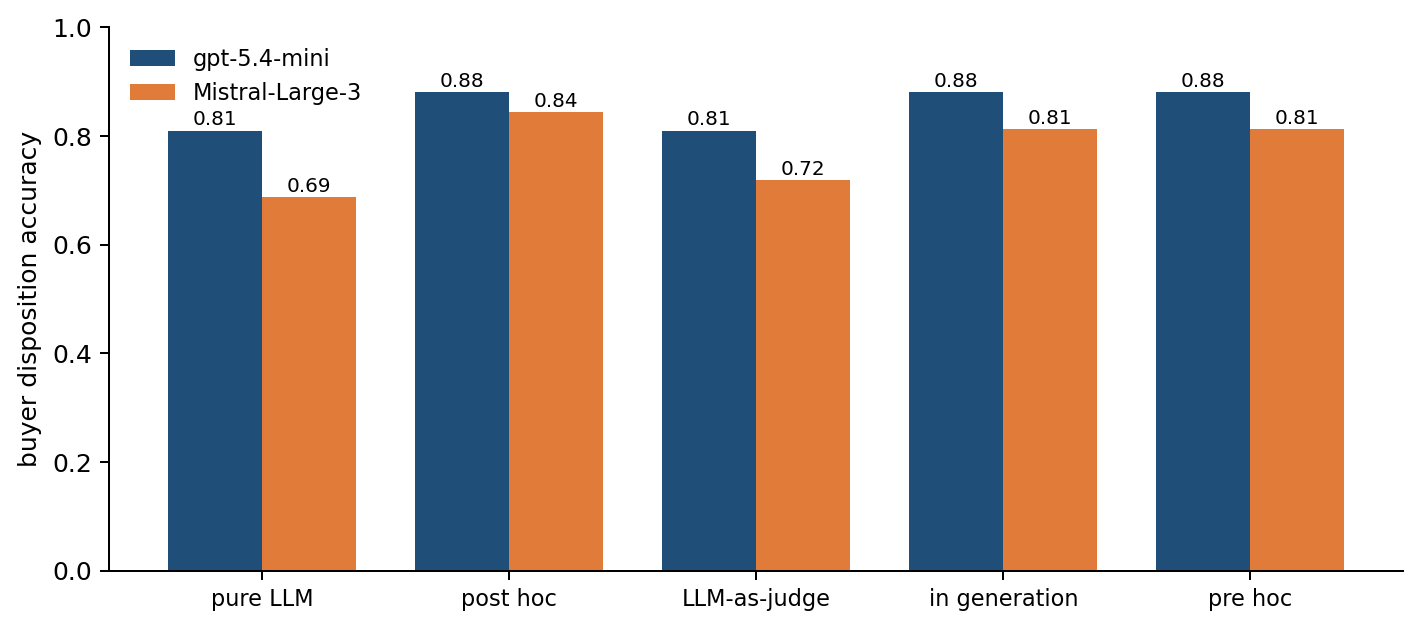
\includegraphics[width=0.82\textwidth]{Figures/fig_mistral_vs_gpt_accuracy.png}
\caption{Per-design disposition accuracy on the 32 buyer cases under the primary model (gpt-5.4-mini) and the second model (Mistral-Large-3).}
\label{fig:app:crossmodel:acc}
\end{figure}

\begin{figure}[htbp]
\centering
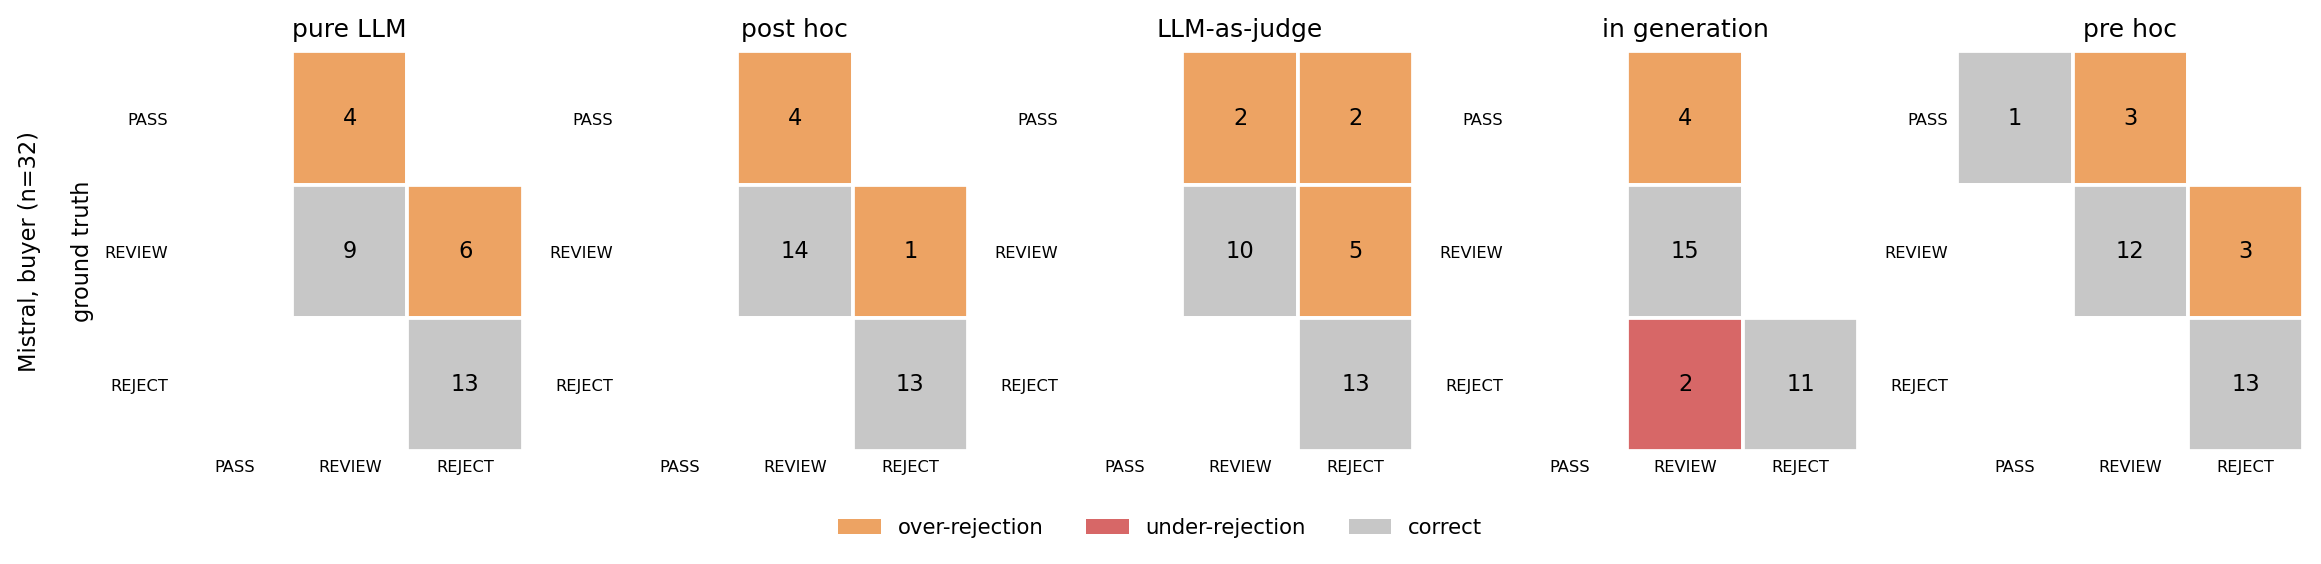
\includegraphics[width=\textwidth]{Figures/fig_mistral_confusion_buyer.png}
\caption{Disposition confusion matrices on the 32 buyer cases under Mistral-Large-3, one panel per design.}
\label{fig:app:crossmodel:conf}
\end{figure}

\begin{table}[htbp]
\centering
\caption{Error direction, reproducibility and per-run latency per design under Mistral-Large-3, buyer cohort (32 cases). Over-rejection routes a sound ASN to manual review; under-rejection lets a defective ASN through. Identical counts cases with the same disposition in all 3 replays.}
\label{tab:app:crossmodel:errors}
\footnotesize
\begin{adjustbox}{max width=\textwidth}
\begin{tabular}{@{}lcccc@{}}
\toprule
\textbf{Design} & \textbf{Over-rejections} & \textbf{Under-rejections} & \textbf{Identical across 3 replays} & \textbf{Median latency (s)} \\
\midrule
pure LLM      & 10 & 0 & 27/32 & 82.3 \\
post hoc      & 5  & 0 & 28/32 & 79.9 \\
LLM-as-judge  & 9  & 0 & 21/32 & 94.4 \\
in generation & 4  & 2 & 25/32 & 102.3 \\
pre hoc       & 6  & 0 & 26/32 & 61.1 \\
\bottomrule
\end{tabular}
\end{adjustbox}
\end{table}

Three patterns from the primary model carry over to the second. First, the safety asymmetry: the post hoc and pre hoc designs make every error in the over-rejection direction, while in generation is again the only design to under-reject, letting 2 defective ASNs through, so the soft enforcer is the first to lose the safety property as the model weakens. Second, the reproducibility order is preserved: LLM-as-judge is the least stable across replays (21/32 identical) and the enforcer-bearing designs the most stable, mirroring the primary model. Third, the operational ranking holds: pre hoc has the lowest latency (61~s median) even on this model. Latency is the one figure that shifts in absolute terms. Every design runs roughly 5 to 8 times slower than the primary model's 7.9 to 13.9~s, so the larger model buys no accuracy here and costs time. The enforcer's protective effect, its safety direction and its stability are therefore properties of the architecture and survive the model swap, while raw accuracy and speed track the model.

\paragraph{Synthetic cohort under the second model.} The second model was also run on the synthetic cohort (67 cases, majority of 3 replays), scored by construction as in Section~\ref{sec:results:synthetic}. Under the per-model tool-use accommodation 27 of the 216 in generation runs (about 12 per cent) returned transport errors; these are outvoted by the majority of 3 replays, so the design is reported on the same basis as the others. Table~\ref{tab:app:crossmodel:syn} reports disposition accuracy, single rule recall over the 41 evaluable targets, and failed PASS controls for the 5 designs.

\begin{table}[htb]
\centering
\caption{Synthetic cohort under Mistral-Large-3 (67 cases, majority of 3 replays): disposition accuracy, single rule recall over the 41 evaluable targets, and failed PASS controls (of 9 single rule clean cases).}
\label{tab:app:crossmodel:syn}
\footnotesize
\begin{tabular}{@{}lcccc@{}}
\toprule
\textbf{Design} & \textbf{Enforcer?} & \textbf{Accuracy} & \textbf{Recall} & \textbf{Failed PASS controls} \\
\midrule
pure LLM      & no  & 0.58 & 17/41 & 8/9 \\
post hoc      & yes & 0.64 & 23/41 & 7/9 \\
LLM-as-judge  & no  & 0.49 & 16/41 & 8/9 \\
in generation & yes & 0.84 & 30/41 & 2/9 \\
pre hoc       & yes & 0.69 & 24/41 & 2/9 \\
\bottomrule
\end{tabular}
\end{table}

Two findings carry over from the primary model. First, the LLM-as-judge design is again the weakest, lowest on both accuracy (0.49) and recall (16 of 41). It fails 8 of the 9 single rule PASS controls, the same over-harshness that collapses it on the primary model, so the collapse replicates across model families. The absolute spread is narrower, because the second model is a weaker fit for the task. Second, the enforcer bearing designs lead on accuracy, with in generation highest on this cohort (0.84). On specificity the picture is mixed: in generation and pre hoc fail only 2 of the 9 PASS controls, while post hoc fails 7, closer to the enforcer free designs. The per-design confusion matrices behind these numbers are shown in Figure~\ref{fig:app:crossmodel:syn:conf}, where under-rejections are more prominent than on the buyer cohort, as expected for a weaker model on the harder synthetic cases.

\begin{figure}[htb]
\centering
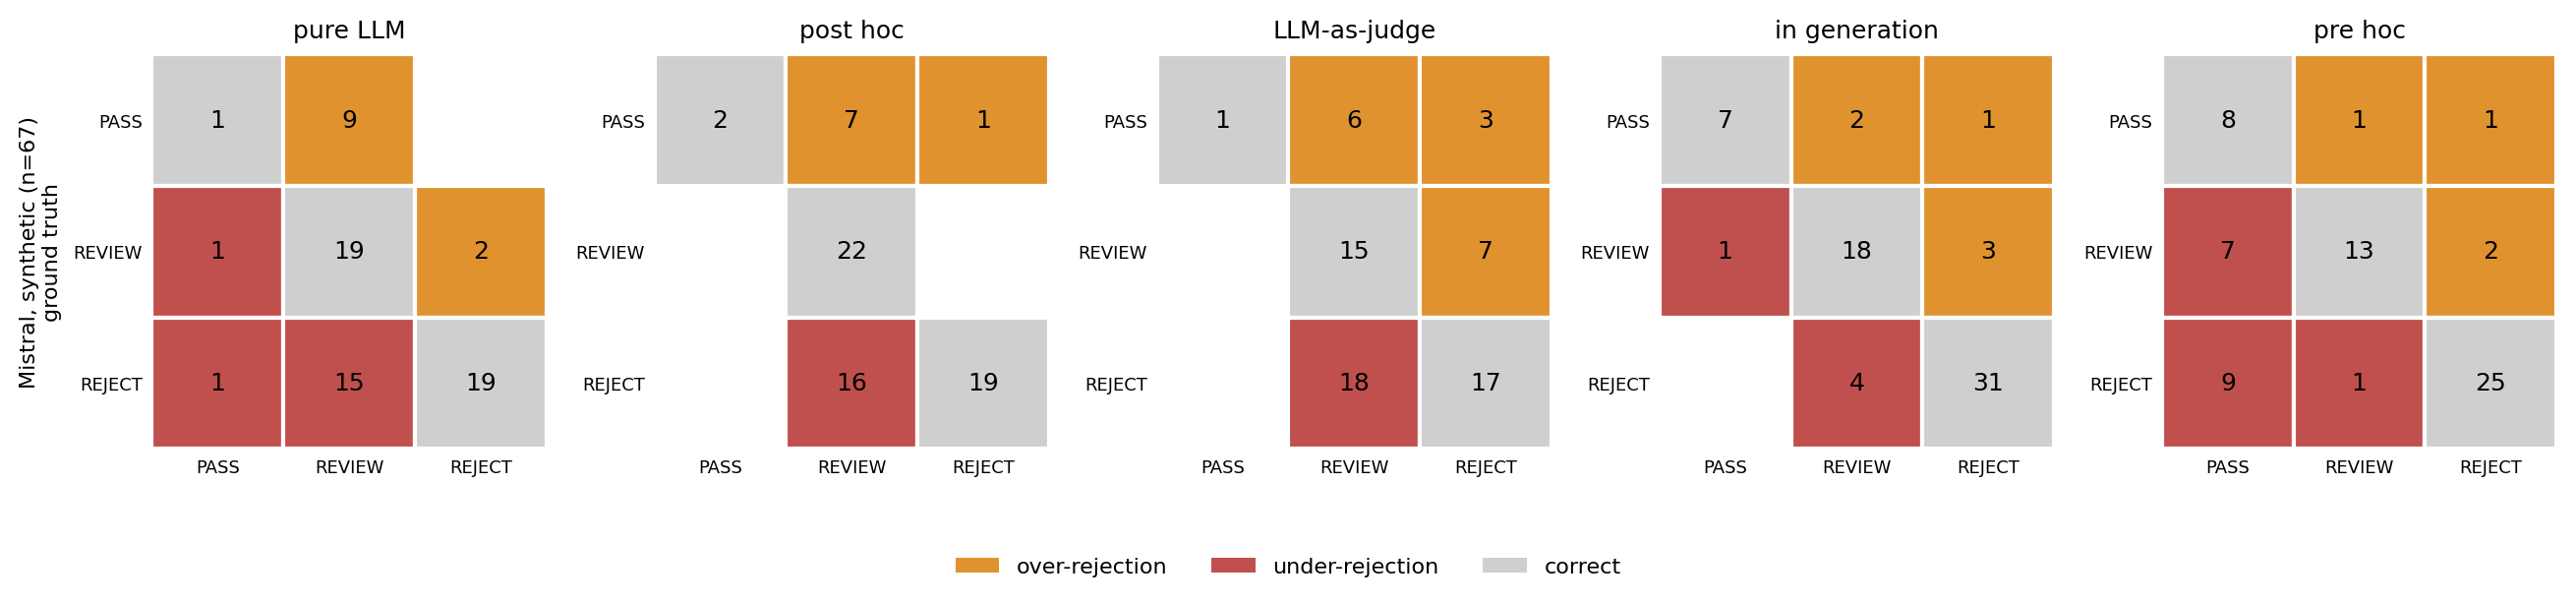
\includegraphics[width=\textwidth]{Figures/fig_mistral_confusion_synthetic.png}
\caption{Disposition confusion matrices on the 67 synthetic cases under Mistral-Large-3, one panel per design. Rows are the by-construction ground truth, columns the pipeline disposition.}
\label{fig:app:crossmodel:syn:conf}
\end{figure}
